\documentclass[a4papaer, 11pt]{article}
%패키지
\usepackage[scale=0.75,twoside,bindingoffset=5mm]{geometry}
\usepackage{kotex} %한글 사용
\usepackage{amsmath} %align 등 기능
\usepackage{graphicx}
\title{GS-WSVM 연구 경과 및 향후 계획 보고}
\author{문종민}

\begin{document}
\maketitle
\abstract{
주요 내용은 아래와 같습니다.
\begin{enumerate}
  
	\item 논문 초안 검토 후 말씀해 주신 주요 사항 3개에 대해 고민해 본 후 내린 결론
	\item Bayesian decision theory 및 SVM asympototics를 도입한 이유 설명 및 논문에 사용할 구체적인 알고리즘 제안
	\item 현재까지 완료된 시뮬레이션 세팅 및 향후 계획
\end{enumerate}
}
\section{교수님의 검토 사항에 대한 고찰}
논문 초안 검토 후 말씀해 주신 주요 사항 3개에 대해 고민해 보고 내린 결론입니다.
\subsection{GMC 기반 undersampling}
\begin{itemize}
	\item 교수님께서 oversampling에 더해 undersampling 또한 결합하는 것을 제안해 주셨고, Weighted Support Vector Machine Using k-Means Clustering 논문을 참고문헌으로 주셨습니다.
	\item Undersampling은 imbalance ratio를 완화시킬 뿐 아니라 SVM의 training과 prediction 속도를 빠르게 하는 장점이 있습니다. 반면, 주어진 데이터를 다 활용하지 못하고 일부를 버리게 되는 것이 단점입니다.
	\item \textbf{(Undersampling 사용 이유)} 논문을 읽어보고, 논문의 checkerboard data를 R로 구현하여 여러 sample size와 imbalance ratio에서 다양한 setting의 SVM을 돌려 본 결과, highly imbalanced large dataset(ex. 약 100:1 이상의 imbalance ratio와 10만개 이상 크기의 데이터셋)에서 SVM에 SVM 적용 시 oversampling과 undersampling의 결합이 유용하겠다는 생각이 들었습니다.
	\begin{enumerate}
		\item \textbf{(학습시간 감소)} SVM의 시간 복잡도가 $O(n^2)$에 달하기 때문에, 	dataset 크기가 커질수록 training, prediction 속도가 급격히 저하합니다. SVM은 제 성능을 내기 위해 하이퍼파라미터 튜닝이 필수적이므로, training 속도의 저하는 치명적입니다. 한 번 training에 1분이 걸린다면, gamma, C를 10개씩만 시도해 본다고 해도 100번의 training을 해야 하니 실질적인 training time은 100분이 됩니다.따라서 undersampling을 통해 dataset 크기 자체를 줄여야 할 필요가 있습니다.
		\item \textbf{(Imbalance ratio 완화)} Oversampling은 데이터에 noise를 더하므로 300\%, 400\% 정도로 많이 하기가 어렵습니다. 따라서 imbalance ratio가 매우 높을 경우, oversampling만으로는 imbalance를 유의미하게 완화하기 어렵습니다. 한편 undersampling만 사용한다면 데이터를 너무 많이 버리게 되므로 문제가 됩니다. 따라서 Undersampling과 oversampling을 조합한다면 두 방법의 단점을 상호보완하면서 imbalance ratio를 많이 낮출 수 있습니다.
		\item \textbf{(GMC가 효과적인 환경)} GMC는 k-means와 달리 데이터의 분산까지 고려하므로 데이터가 많이 필요한데, Highly imbalanced and large dataset일 경우, negative sample의 수가 매우 많게 됩니다. 따라서 negative sample에 GMC가  잘 학습될 수 있고, 이를 통해 k-means 기반 undersampling보다 데이터에 대해 더 많은 정보를 고려하여 undersampling을 하는 것이 되므로 성능이 더 잘 나올 수도 있습니다.
	\end{enumerate}
	
	\item \textbf{(결론)} 따라서 기존의 oversampling + wsvm에 더하여 undersampling을 하는 것까지 포함하여 시뮬레이션을 해 보고 성능을 비교해 보기로 결정하였습니다.
	
\end{itemize}	
\subsection{Weighted SVM의 boundary가 별로 왜곡되지 않을 수도 있음}
\begin{itemize}

\item 교수님께서 KKT condition에 의해 weighted SVM에서 positive support vector가 감소하더라도, 실제로는 boundary 모양이 별로 왜곡되지 않을 수 있다고 지적해 주셨습니다.
\item 실제로 checkerboard 데이터를 가지고 여러 상황에서 SVM의 decision boundary를 그려 본 결과, boundary가 별로 왜곡되지 않았습니다.
\item \textbf{(왜곡이 나타나지 않는 이유)}제가 boundary 왜곡에 대해 idea를 얻었던 Wu et al., 2003 논문에서 boundary의 왜곡이 나타나는 예제는 imbalance ratio가 10000:1로 매우 높고, 정사각형 안에 uniform 분포를 사용해 만든 checkerboard 데이터를 사용하여 ideal boundary가 직선이었던 상황이었습니다. Imbalance ratio가 더 낮고 ideal boundary가 직선이 아닌 상황에서는 boundary 왜곡이 잘 일어나지 않는 것으로 보입니다.
\item \textbf{(결론)} 제가 boundary 왜곡을 언급한 이유는 WSVM의 단점을 찾아내서 WSVM에  resampling을 결합하는 것을 정당화하기 위해서였습니다. WSVM에 단점이 없다면 굳이 (명확한 단점이 있는) resampling을 결합할 필요가 없다고 생각했기 때문이었습니다. 하지만 교수님이 주신 논문을 읽고, 논의의 방향을 바꾸어 resampling의 단점(데이터의 손실과 노이즈 발생)을 보완하기 위해 WSVM을 사용한다는 논리를 사용하기로 하였습니다.
\end{itemize}
\subsection{GMC oversampling은 원본의 likelihood를 보존한다고 볼 수 없음}
\begin{itemize}
	\item GMC 또한 정규분포를 가정하는 것이기에 원본분포와 항상 비슷하다고는 할 수 없다고 말씀해 주셨습니다.
	\item 비록 GMC가 샘플 수와 클러스터 수가 무한히 커진다면 모든 연속형 분포를 근사할 수 있지만, 실제 분석에서 positive sample은 개수가 적을 뿐 아니라 cluster 수도 무한히 늘리지 않으므로, GMC oversampling을 한 데이터는 원본 분포와 항상 비슷하다고 하기는 어려운 것이 맞습니다.
	\item \textbf{(결론)} 논문에서 GMC oversampling이 원본 분포를 근사한다는 내용을 빼고, oversampling이나 undersampling시 원본 분포가 보존되지 않음을 언급하겠습니다.

\end{itemize}

\section{Bayesian decision theory 및 SVM asymptotics를 도입한 이유}
\subsection{Resampling과 wsvm결합 시 가이드라인의 필요성}
\begin{itemize}
	\item SVM에 resampling 과 WSVM을 둘 다 적용하는 연구는 많지만, resampling을 얼마나 하고 weight를 어떻게 주어야 원하는 결과를 얻을 수 있는지에 대해 통계학 이론에 기반한 가이드라인을 제시한 경우는 별로 없습니다.
	\item Benchmark dataset에서의 성능이 아니라 통계학 이론에 기반한 가이드라인을 만들기 위해 Bayesian decision theory와 SVM asymptotics를 도입했습니다. 가이드라인의 대략적인 내용은 아래와 같습니다.
	\begin{enumerate}
		\item Bayesian decision theory를 기준으로 한 최적의 분류기를 Bayes rule이라 합니다.
		\begin{itemize}
			\item Bayes rule을 정의하기 위해서는 false positive와 false negative의 cost ratio가 주어져 있어야 합니다. 예를 들어, 암 양성을 음성으로 판정했을 때 발생하는 비용이 음성을 양성으로 판정했을 때의 비용의 100배 정도라는 정보가 있어야 합니다.
		\end{itemize}

		\item 계산 비용 등을 고려하여 데이터에 resampling을 적용해 imbalance ratio를 완화합니다.
\begin{itemize}
	\item WSVM으로 class 내부 뿐 아니라 class 간 weight 비율도 조절할 것이므로, 1:1까지 낮추지 않고 적당한 수준까지만 낮춥니다.
\end{itemize}
		\item 완화된 정도를 반영하여 Lin et al., 2002의 방법대로 weight를 정해서 WSVM을 적용하면, 그 결과는 $n\to \infty$일 때 1.의 Bayes rule로 수렴합니다.
			\begin{itemize}
				\item Lin et al., 2002의 증명은 본래 resampling이 아니라 계획적인 sampling bias를 전제로 합니다.
				\item \textbf{(계획적인 sampling bias 설명)} 예를 들어, 100명의 sample을 뽑는 암 관련 연구에서 전체 인구에서 정상인과 암환자 비율이 10:1인 상황을 가정합니다. Sample에 암환자가 너무 적은 것을 염려하여 표본 추출 단계에서 암 환자 집단에서 50명을 랜덤 추출하고, 정상인 집단에서 50명을 랜덤 추출한다면, class 비율만 1:1로 변경되고 class별 분포는 동일하게 됩니다.
				\item \textbf{(이 방법의 한계)} 하지만 GMC 기반 resampling은 class별 원본 분포를 보존하지 못합니다. 따라서 이 방법은 절대적인 기준이 될 수 없으며 heuristic에 불과합니다.
				\item \textbf{(이 방법의 의의)} 그러나 거의 모든 resampling+wsvm 연구들이 weight를 정할 때 heuristic을 사용하거나 아예 결정 기준을 제시하지 않습니다. 또한 heuristic을 제시한 경우에도 그것이 통계학 이론에 기반한 경우는 거의 없었습니다. 따라서 저는 이 방법이 의미가 있다고 판단하였습니다.
				\item Lin et al., 2002의 증명은 weight를 class별로 할당하는 방법에 대한 것입니다. 하지만 증명을 약간 수정하면, class별 weight합이 유지된다는 가정 하에 weight를 세 종류로 주는 법, 더 나아가서 training sample마다 weight를 다르게 주는 방법에 대해서도 같은 결과가 성립함을 보일 수 있습니다.
			\end{itemize}
	\end{enumerate}
	\item 즉, resampling을 먼저 하고 그에 맞추어 weight를 정하는데, weight를 정할 때 Bayes rule이 보존되도록 한다는 것입니다. Bayes rule이라는 목표를 설정했기 때문에 resampling결과에 맞추어 weight를 정하는 법을 구체적으로 제시할 수 있게 되었습니다.
	\item \textbf{(문제점)} Class 간 weight 차등 적용, negative class 내 weight 차등 적용은 구체적인 방법을 제시하였지만, positive class 내에서 original sample과 synthetic sample 간 weight를 차등 적용할 구체적인 방법을 아직 생각해 내지 못하였습니다.
\end{itemize}

 \subsection{구체적인 알고리즘 제안}
 \begin{enumerate}
 	\item [Step 1.] Tuning parameter set에서 paramter 조합을 하나 정합니다. Parameter set은 gamma, lambda(or C), oversampling/undersampling rate, positive data에서 original/synthetic weight ratio의 값으로 구성됩니다.
 	\item [Step 2.] Positive class에서 BIC를 기준으로 GMC를 학습하고, 학습한 모델에서 Step 1에서 정한 rate에 따라 oversampling합니다.
 	\item [Step 3.] Negative class에서 Step 1에서 정한 rate에 맞춰 cluster 개수를 정해 GMC를 학습하고, cluster center만 남기고 나머지 데이터를 버립니다. 각 cluster의 size도 저장합니다. Cluster size를 계산하기 위해 각 sample $x$의 cluster membership을 정할 때는 $Pr(cluster|x)$가 최대가 되는 cluster를 선택합니다.
 	\item [Step 4.] Lin et al., 2002의 방법을 사용해 positive와 negative class에 적용될 weight을 계산합니다.
 	\item [Step 5.] Class별로 Step 4에서 계산한 weight의 총합을 유지하면서 세부적인 weight 조정을 합니다. positive class에서는 Step 1에서 정한 ratio를 사용해 original/synthetic sample의 weight를 조절합니다. negative에서는 cluster size에 비례하도록 각 cluster center의 weight를 조절합니다.
 	\item [Step 6.] SVM을 수행하고 error를 계산합니다.
 	\item [Step 7.] Step 1-6을 반복하여 최적의 parameter set을 찾아냅니다.
 	\end{enumerate}

\section{시뮬레이션 계획}
\subsection{현재까지 완료한 사항}
아직 본격적으로 시뮬레이션을 시작하지는 못했습니다. 현재까지 완료한 사항은 아래와 같습니다.
\begin{enumerate}
	\item 교수님 논문의 checkerboard 데이터를 사용하기로 하고, sample size, imbalance ratio, mean과 sigma를 바꿔 가면서 데이터를 편리하게 생성할 수 있는 함수를 만들었습니다.\\
	
	\item 생성한 데이터를 시각화하고, Bayes rule의 계산과 boundary 시각화를 수행하는 함수를 만들었습니다. SVM의 boundary 또한 그릴 수 있습니다. Bayes rule만 그린 결과물은 아래와 같은 형태입니다.\\
	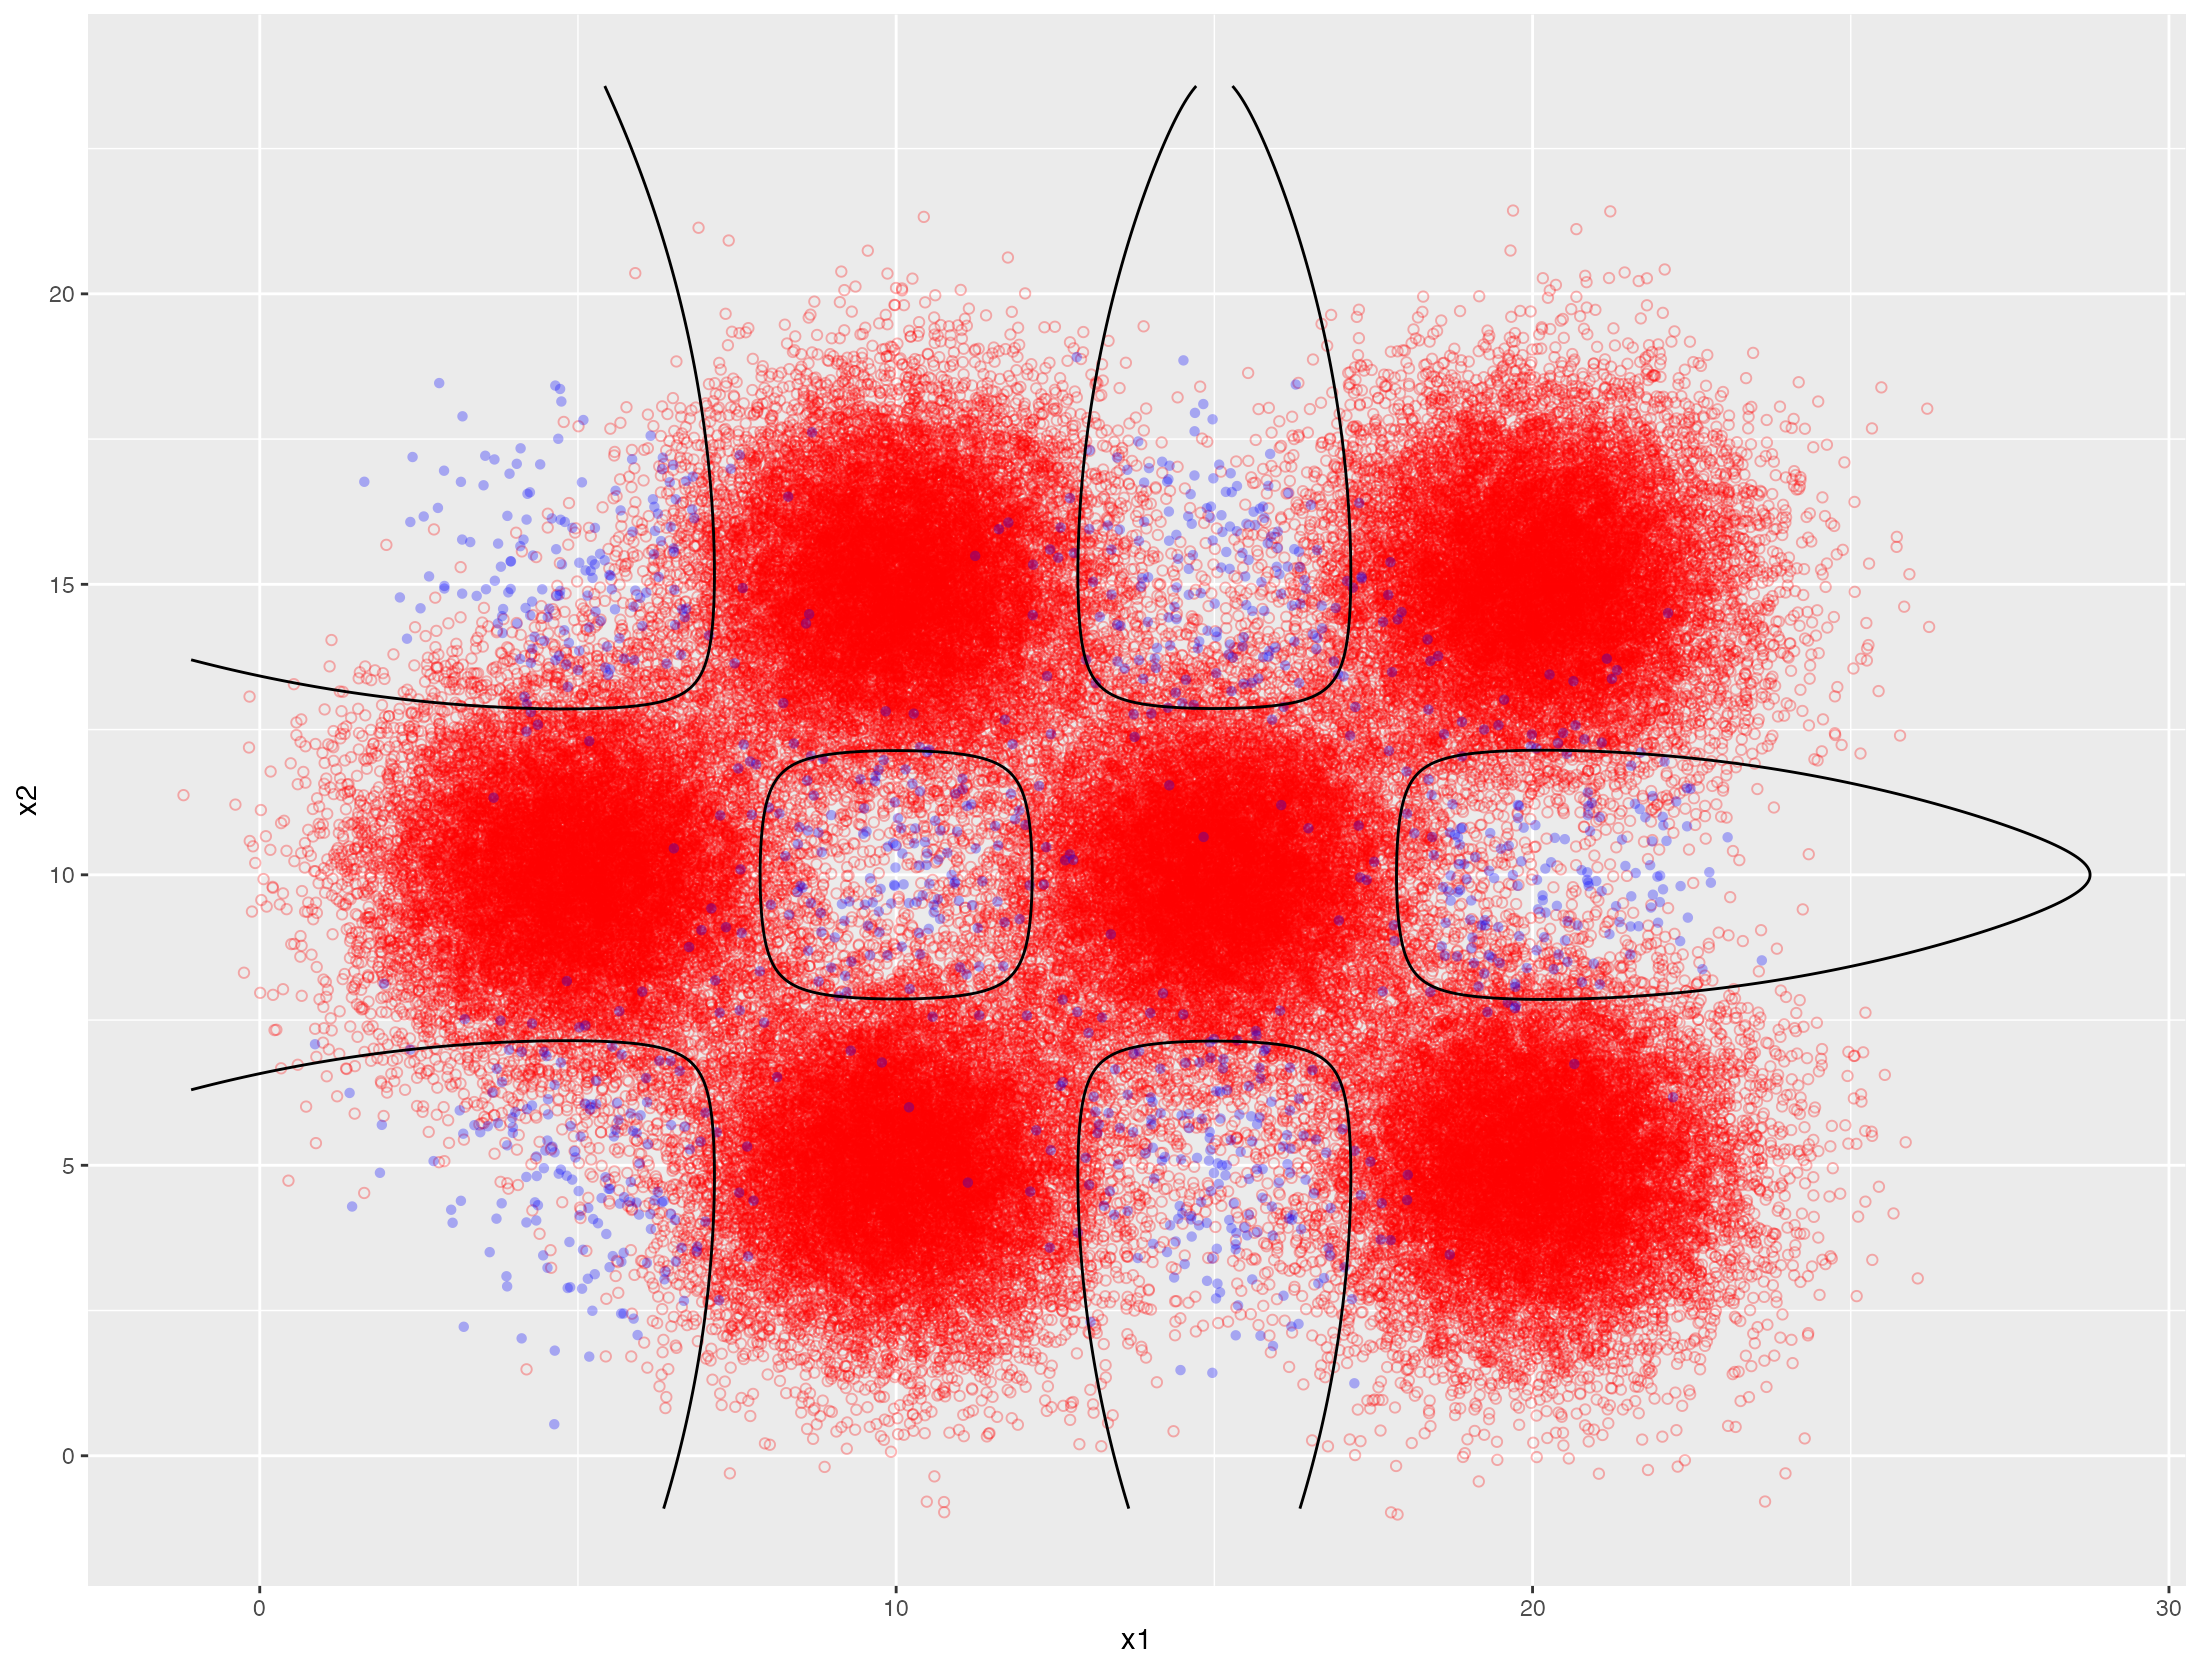
\includegraphics[width=0.8\textwidth]{checkerboard}
	
	\item 분류기의 test set 성능을 accuracy, sensitivity, precision, specificity, g-mean으로 평가하는 함수를 만들었습니다.
\end{enumerate}

\subsection{앞으로의 계획}
\begin{itemize}
	\item 여러 imbalance ratio 및 sample size에서 2.2의 알고리즘을 돌려 보면서 적절한 시뮬레이션 세팅을 찾고 시뮬레이션을 완료하겠습니다.
	\item gmc oversampling에서 original sample과 synthetic sample 간 적절한 weight 차등적용 방법에 대해 고민해보겠습니다. 혹시 이 사항에 대해 좋은 의견이 있으시면 조언 부탁드립니다.
	\item 시뮬레이션 완료 후 논문 본문을 작성하겠습니다.
\end{itemize}

\end{document}
